\apendice{Anexo de sostenibilización curricular}

\section{Introducción}

Naciones Unidas define el Desarrollo Sostenible en \cite{ONU-ODS} con el objetivo de erradicar la pobreza, proteger el planeta y asegurar la prosperidad para todos en un plazo de 15 años. Este plan se compone de 17 objetivos llamados ODS visibles en \ref{fig:sost_1}, y está incluido en la Agenda 2030, entrando en vigor el 1 de enero de 2016. Se han estudiado las asociaciones de este estudio con los OMS, estimando una especial asociación con tres de ellos, a partir de los que se muestran las siguientes consideraciones.

En primer lugar, y de forma más significativa, este estudio fomenta la salud y el bienestar del desarrollo sostenible. La comprensión, así como el avance en el conocimiento de la interacción entre la glucosa y la insulina contribuye a la mejora de la comprensión de estos sistemas, lo que a su vez conlleva al desarrollo de nuevos avances, tanto en el ámbito preventivo, como en el tratamiento, así como en la tecnología. Especial relevancia tiene, para este objetivo, la aparición de nuevos mecanismos de control de la diabetes, que pueden mejorar considerablemente el pronóstico y nivel de vida de todas las personas afectadas. Concretamente, la investigación en este campo es clave para varios aspectos. En primer lugar, la diabetes es una enfermedad crónica que puede causar numerosas complicaciones si no se trata de manera adecuada (enfermedades cardiovasculares, cardiopatía o nefropatía, entre otras). El aumento de conocimiento sobre esta patología funciona como técnica eficaz para la prevención, parte fundamental en la salud pública. Por otro lado, el desarrollo de nuevas soluciones tecnológicas, así como el descubrimiento de datos reveladores puede tener un impacto significativo en los tratamientos de la enfermedad. Esto repercute directamente en los pacientes, que podrían experimentar mejoras muy significativas en su calidad de vida, minimizando además el riesgo de complicaciones. Además, el avance médico implica la promoción de bienestar no solo para el paciente individual, sino para toda la población, independientemente de su edad, género, origen o situación socioeconómica. La expansión de estas mejoras contribuye a la universalidad del acceso a ellas. El ejercicio físico promueve la promoción de un estilo de vida activo y saludable, mostrando las mejoras que se producen al llevarlo a cabo. De esta manera, no solo se mejora la salud cardiovascular y muscular, sino que se puede reducir el riesgo de complicaciones, eje de la importancia de la salud.

Por otro lado, también se puede asociar, en menor grado, este estudio con el objetivo número 12 del Desarrollo Sostenible: Producción y Consumo responsables. Además de concienciar a la población sobre los riesgos que acarrea la enfermedad de la diabetes, aumentar la información sobre este campo permite reducir el tamaño del problema, centrando las estrategias de creación de nuevos sistemas. De esta manera se contribuye a la reducción de desperdicio de recursos médicos, así como a la optimización de su uso para tratamientos más eficientes. Este desperdicio de recursos, entre los que podrían destacar la fabricación de medicamentos y los dispositivos médicos, puede tener un impacto significativo en el medio ambiente, por lo que su reducción contribuye directamente con el consumo responsable. 

Por último, el objetivo número 9, de Industria, innovación e Infraestructura, se relaciona directamente con el desarrollo de nuevos avances, especialmente tecnológicos, de mecanismos de monitorización y control de los sistemas glucorregulatorios, como son el caso de las bombas de insulina y del páncreas artificial. Estos avances representan una forma de innovación en el campo de la medicina, así como en la gestión de enfermedades crónicas, contribuyendo al avance de la ciencia. La infraestructura, pasa primero por el aprendizaje profundo de la interacción entre la glucosa y la insulina, así como por el descubrimiento de nuevas posibles relaciones que contribuyan a la mejora de la enfermedad, especialmente en cuanto a tratamiento de la patología. La creación de estos sistemas tecnológicos contribuye, por su parte, a la creación de nuevas empresas y fomento de la industria. El fortalecimiento de la infraestructura también repercute en la atención médica, pues el desarrollo de nuevas técnicas puede reducir la duración de tratamientos, así como la duración de consultas y estudios del paciente. Al aplicar este hecho al conjunto de la sociedad, se mejora el acceso a servicios de salud de calidad, y disminuyen los conflictos médicos respecto a pocos recursos y diagnósticos.

\begin{figure}[htbp]
    \centering
    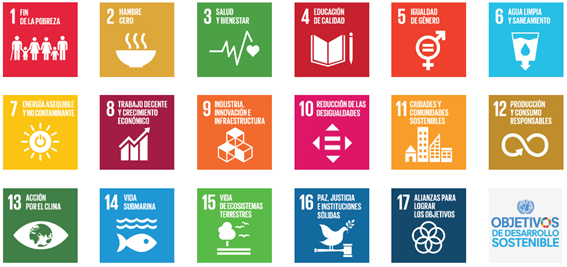
\includegraphics[width=0.9\linewidth]{img/anexos/sostenibilidad/sostenibilidad.png}
    \caption{Objetivos ODS del Desarrollo Sostenible. }
    \label{fig:sost_1}
\end{figure}